\chapter{构建、运行与测试}

WaterOS的验证从同一套Makefile入口开始。构建参数决定目标架构、内核配置、CPU数量和
根文件系统，Guest中的测试脚本再覆盖系统调用、进程、内存、文件和网络等路径。本章先
说明如何得到可运行环境，再给出测试方法和已经保存的测试结果。性能数字只用于
描述本次QEMU配置下的运行情况，不与裸机或其他操作系统作未经控制的横向比较。

\section{构建与运行}

内核构建入口统一处理Cargo feature、内核文件名、用户镜像和QEMU参数。常用参数为
\code{ARCH=rv|la}、\code{PROFILE=pre|final}与\code{SMP}。\code{pre}用于初赛镜像及其
自动测试队列，\code{final}用于完整用户环境；两种profile选择的根文件系统和启动任务不同，
因此测试记录必须同时写明架构与profile。

\begin{table}[htbp]
  \centering
  \caption{主要构建与运行入口}
  \label{tab:build-entry}
  \begin{tabularx}{\textwidth}{L{3.0cm}L{4.8cm}Y}
    \toprule
    目标 & 示例命令 & 用途 \\
    \midrule
    查看配置 & \code{make show-config ARCH=rv PROFILE=final SMP=8} & 确认目标架构、镜像、
    feature和QEMU参数。\\
    静态检查 & \code{make check ARCH=rv PROFILE=final} & 检查目标架构上的类型、依赖与
    条件编译组合。\\
    构建内核 & \code{make build ARCH=rv PROFILE=final} & 生成对应架构和profile的内核镜像。\\
    自动运行 & \code{make run ARCH=rv PROFILE=pre SMP=8} & 启动Guest并执行镜像预置的测试队列。\\
    交互运行 & \code{make shell ARCH=rv PROFILE=final SMP=8} & 进入串口shell，执行定向测试
    或应用演示。\\
    \bottomrule
  \end{tabularx}
\end{table}

双架构构建应分别执行，不能以RISC-V64结果代替LoongArch64结果。日常测试默认使用QEMU
snapshot，Guest对磁盘的修改不会写回基础镜像；需要检查持久化结果时，应复制基础镜像，
再显式设置\code{WRITE\_DISK=1 SNAPSHOT=0}。若QEMU提示\code{hostfwd}端口已占用，应先
释放端口或修改转发配置，这属于宿主运行环境冲突，不是内核编译错误。

\begin{bashcode}
make check ARCH=rv PROFILE=final
make check ARCH=la PROFILE=final
make build ARCH=rv PROFILE=final
make build ARCH=la PROFILE=final

# 自动测试与交互环境
make run   ARCH=rv PROFILE=pre   SMP=8
make shell ARCH=rv PROFILE=final SMP=8
\end{bashcode}

\section{测试方法}

测试按“能否构建、能否启动、接口是否正确、完整负载能否结束”逐层进行。上一层通过只是
进入下一层的前提。例如，脚本返回0说明测试队列执行完毕，但仍需查看每个测试程序自己的
结果；性能程序能够输出数字，也不能代替功能测试和长期稳定性检查。

\begin{longtable}{L{2.8cm}L{5.2cm}L{5.3cm}}
  \caption{测试层次与判定方法}\label{tab:test-method}\\
  \toprule
  层次 & 测试内容 & 判定依据 \\
  \midrule
  \endfirsthead
  \toprule
  层次 & 测试内容 & 判定依据 \\
  \midrule
  \endhead
  构建检查 & RISC-V64和LoongArch64的\code{check/build}，分别覆盖pre与final配置。 &
  构建进程正常退出，目标文件生成，feature组合与预期一致。\\
  启动检查 & 1核、8核启动，挂载根文件系统并进入自动队列或交互shell。 & BSP与AP完成
  初始化，根文件系统可访问，用户态首进程能够运行。\\
  功能回归 & BusyBox、libctest、LTP及定向系统调用程序。 & 以测例自身的断言、退出状态
  和分项汇总为准，不用测试脚本的总退出码覆盖分项失败。\\
  综合负载 & CAgent、BuildStorm、libc-bench、lmbench、iozone和stress-ng。 & 工作负载
  完整结束，随后仍能创建进程、读写文件并执行shell命令。\\
  应用演示 & Nano-X桌面、图形终端、输入设备和Doom。 & framebuffer与evdev可用，窗口
  能创建和刷新，键鼠事件及PTY输入能够到达用户程序。\\
  \bottomrule
\end{longtable}

自动测试日志由测试组起止标记和runner记录组成。统计时先确认每个测试组同时出现
\code{START}与\code{END}，再检查程序退出状态和组内结果。LTP会为不同用例分别输出
\code{Summary}，不能把这些局部统计直接累加；否则同一批累计数字会被重复计算。原始串口
日志应与内核commit、用户镜像摘要、QEMU版本和完整命令一同保存。

\section{当前测试数据}

\subsection{系统调用与基准测试}

表\ref{tab:current-log-groups}来自一次保存完整的串口测试记录。该记录使用
\code{ARCH=rv PROFILE=pre SMP=8}运行，Preliminary镜像依次执行了五个测试组。五条runner
命令均以退出码0结束，测试队列从启动第一个程序到最后一项结束约14分28秒。这里的“完成”
表示程序返回并留下完整结果，不等同于其中每个子测例都通过。

\begin{table}[htbp]
  \centering
  \caption{本次自动测试包含的测试组}
  \label{tab:current-log-groups}
  \begin{tabularx}{\textwidth}{L{3.5cm}C{2.4cm}L{3.0cm}Y}
    \toprule
    测试组 & 运行时间 & runner状态 & 日志中可确认的结果 \\
    \midrule
    cyclictest-glibc & 20.794 s & exit 0 & 无负载/有负载、1线程/8线程四组均运行结束。\\
    ltp-musl & 369.519 s & exit 0 & 调度341个不同的LTP用例并到达测试组结束标记。\\
    libcbench-glibc & 10.098 s & exit 0 & malloc、字符串、线程、stdio、UTF-8和正则项目完成。\\
    lmbench-glibc & 340.408 s & exit 0 & 系统调用、进程、pipe、缺页等延迟项目完成。\\
    iozone-glibc & 127.237 s & exit 0 & 4进程文件I/O测试完成并输出吞吐量。\\
    \bottomrule
  \end{tabularx}
\end{table}

表\ref{tab:lmbench-result}列出lmbench日志中较容易复核的项目。所有值都来自QEMU中的本次
运行，单位为微秒；它们适合用于同一环境下修改前后的回归比较。

\begin{table}[htbp]
  \centering
  \caption{本次lmbench部分延迟数据}
  \label{tab:lmbench-result}
  \begin{tabularx}{\textwidth}{L{4.2cm}C{2.8cm}L{4.2cm}C{2.8cm}}
    \toprule
    项目 & 延迟/\textmu s & 项目 & 延迟/\textmu s \\
    \midrule
    简单系统调用 & 31.0560 & 简单read & 59.9029 \\
    简单write & 72.9876 & 简单stat & 233.2609 \\
    pipe往返 & 378.7794 & 保护异常 & 259.0301 \\
    fork后退出 & 1757.2500 & fork后execve & 2027.3333 \\
    文件缺页 & 69.8401 & 打开并关闭文件 & 501.9091 \\
    \bottomrule
  \end{tabularx}
\end{table}

iozone使用4个并发进程、1 MiB文件和1 KiB记录。表\ref{tab:iozone-result}采用日志中的
children aggregate值，避免把单进程最小值与总吞吐量混在一起。

\begin{table}[htbp]
  \centering
  \caption{本次iozone部分吞吐量数据}
  \label{tab:iozone-result}
  \begin{tabularx}{\textwidth}{L{5.0cm}C{3.1cm}Y}
    \toprule
    项目 & 吞吐量/(KiB/s) & 测试说明 \\
    \midrule
    4进程首次写入 & 2523.87 & 普通write路径，1 KiB记录。\\
    4进程顺序读取 & 34926.56 & 普通read路径，读取已有文件。\\
    4进程pwrite & 36041.69 & 按偏移写入。\\
    4进程pread & 38778.26 & 按偏移读取。\\
    \bottomrule
  \end{tabularx}
\end{table}

\FloatBarrier
\subsection{双架构综合负载}

另一组Final镜像测试分别在RISC-V64和LoongArch64上运行CAgent与BuildStorm。RISC-V64
配置为8个虚拟CPU和16 GiB内存，LoongArch64配置为12个虚拟CPU和36 GiB内存。两组配置
并不相同，因此表\ref{tab:dual-arch-workloads}中的时间只用于说明负载完整运行，不用于比较
两种架构的性能。

CAgent启动本地HTTP服务，通过请求触发模板推理和系统操作。十个用例覆盖CPU信息、磁盘
使用、日期、阶乘、文件创建、文件读写、内核信息、文件搜索、目录操作和网络连接。两种
架构均输出十条success记录，测试组正常结束且runner退出码为0。

BuildStorm先检查Rust工具链并执行最小构建，再以multi模式编译ArceOS HelloWorld。该过程
会密集使用进程创建、\code{execve}、文件映射、目录遍历、并发文件读写和内存分配。编译
结束后，脚本继续启动生成的内核产物，以免把“文件已经生成”误判为“产物可以运行”。两种
架构的工具链检查、最小构建、正式编译和产物启动均返回OK。

\begin{table}[htbp]
  \centering
  \caption{双架构CAgent与BuildStorm测试结果}
  \label{tab:dual-arch-workloads}
  \begin{tabularx}{\textwidth}{L{4.4cm}C{4.1cm}C{4.1cm}}
    \toprule
    项目 & RISC-V64 & LoongArch64 \\
    \midrule
    Final运行配置 & 8 vCPU，16 GiB & 12 vCPU，36 GiB \\
    CAgent通过情况 & 10/10 & 10/10 \\
    CAgent测试组耗时 & 5.830 s & 3.661 s \\
    BuildStorm模式 & multi，8 cores & multi，12 cores \\
    BuildStorm计时构建 & 2142.57 s & 1855.00 s \\
    生成产物大小 & 1681000 bytes & 1714568 bytes \\
    产物启动 & OK & OK \\
    两个测试组runner状态 & exit 0 & exit 0 \\
    \bottomrule
  \end{tabularx}
\end{table}

这组结果补充了pre自动队列未覆盖的完整应用路径：CAgent侧重服务进程、socket与文件操作，
BuildStorm侧重用户态工具链、多进程编译和持续文件I/O。它们共同表明两种架构都能够在
Final用户环境中完成较长执行链，而不仅是启动到shell或通过单个系统调用测例。

\FloatBarrier
\section{Nano-X图形演示}

Nano-X适合作为综合功能测试，而不只是界面展示。桌面启动会经过VirtIO GPU、framebuffer
mmap、evdev、VFS设备节点和Unix socket；\code{nxterm}进一步覆盖UNIX98 PTY、shell、
\code{poll/select}与信号；Doom则持续产生窗口刷新和输入事件。因而一次可交互的图形演示
可以同时检查驱动、文件系统、进程和IPC路径。

RISC-V64图形镜像和内核可按以下方式启动：

在用户空间构建环境中生成图形根文件系统：

\begin{bashcode}
make image ARCH=rv PACKAGE=graphics
\end{bashcode}

随后在内核构建环境中指定生成的镜像并启动：

\begin{bashcode}
make shell ARCH=rv PROFILE=pre SMP=8 \
  SDCARD=$ROOTFS_IMAGE \
  EXTRA_FEATURES=user-graphics
\end{bashcode}

进入串口shell后，先启动Nano-X server和桌面，再分别检查终端与Doom：

\begin{bashcode}
start-nanox >/tmp/nanox.log 2>&1 &
nxterm &
start-doom
\end{bashcode}

\begin{figure}[htbp]
  \centering
  \begin{minipage}[t]{0.48\textwidth}
    \centering
    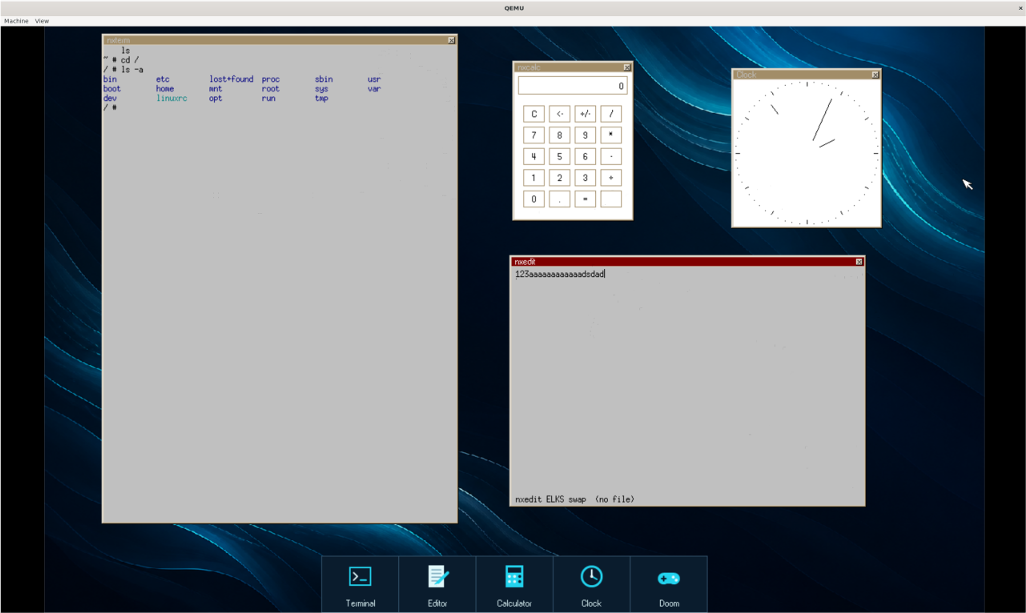
\includegraphics[width=\linewidth]{pic/nanox.png}
    \par\small Nano-X桌面与图形应用
  \end{minipage}
  \hfill
  \begin{minipage}[t]{0.48\textwidth}
    \centering
    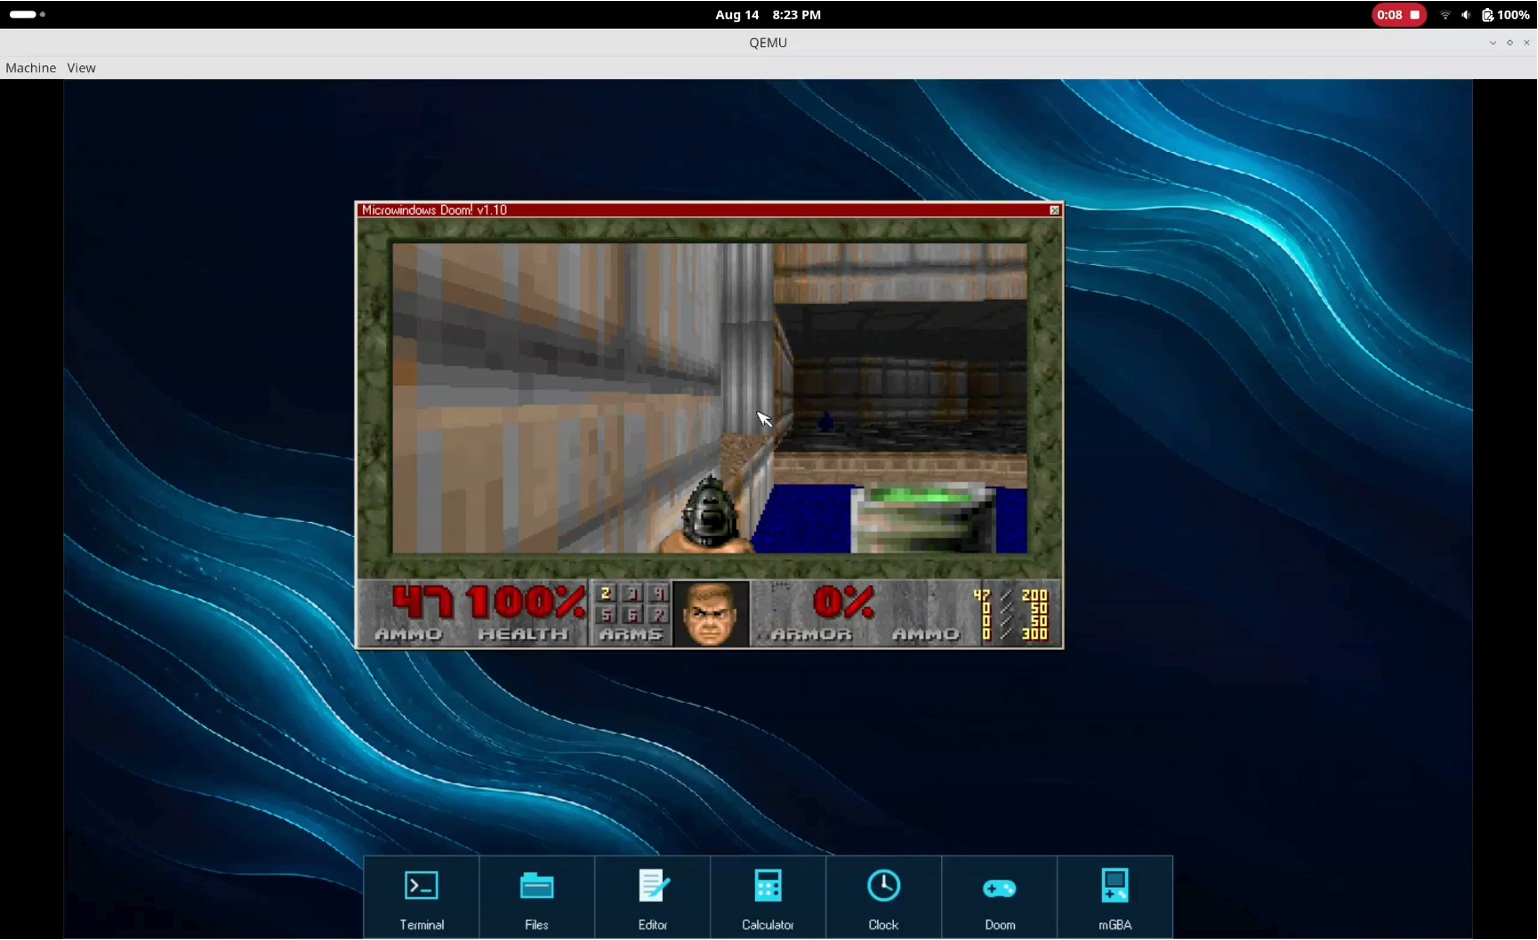
\includegraphics[width=\linewidth]{pic/doom.png}
    \par\small Doom运行画面
  \end{minipage}
  \caption{Nano-X图形环境与Doom应用演示}
  \label{fig:nanox-doom-demo}
\end{figure}
\FloatBarrier

演示时应记录四项现象：桌面是否完整显示；键盘和指针能否操作窗口；\code{nxterm}中能否
执行shell命令并响应Ctrl-C；Doom能否持续刷新并接收输入。需要量化图形路径时，可以使用
\code{NANOX\_STATS=1}和\code{DOOM\_STATS=1}输出提交次数、像素量和FPS。当前
本次自动测试记录不包含图形测试，因此Nano-X应作为独立演示记录，不并入表
\ref{tab:current-log-groups}的五项结果。
